\documentclass[10pt]{acmsiggraph}          % final
%\documentclass[review]{acmsiggraph}      % review
%\documentclass[widereview]{acmsiggraph}  % wide-spaced review
%\documentclass[preprint]{acmsiggraph}    % preprint

%% Uncomment one of the four lines above depending on where your paper is
%% in the conference process. ``review'' and ``widereview'' are for review
%% submission, ``preprint'' is for pre-publication, and ``final'' is for
%% the version to be printed.

%% These two line bring in essential packages: ``mathptmx'' for Type 1 
%% typefaces, and ``graphicx'' for inclusion of EPS figures.

\usepackage{mathptmx}
\usepackage{graphicx}

%% Personal packages I'm using for graphics layout

\usepackage{subfigure}
\usepackage{wrapfig}

%% use this for zero \parindent and non-zero \parskip, intelligently.

\usepackage{parskip}

%% If you are submitting a paper to the annual conference, please replace 
%% the value ``0'' below with your OnlineID. If you are not submitting this
%% paper to the annual conference, you may safely leave it at ``0'' -- it 
%% will not be included in the output.

%\onlineid{0}

%% need to document this!

\acmformat{print}

%% Paper title.

\title{An Analysis of Fragmentation Using Pen Speed and Curvature}

%% Author and Affiliation (multiple authors).

\author{Aaron Wolin\\ Harvey Mudd College\\ awolin@hmc.edu}

%% Keywords that describe your work.
\keywords{Sketch Preprocessing, Noise filtering, Pen computing, Fragmentation}

%%%%%% START OF THE PAPER %%%%%%

\begin{document}

%\teaser{
%  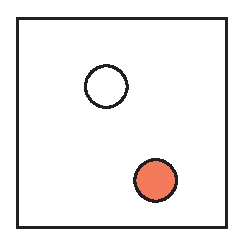
\includegraphics[width=1.5in]{sample.eps}
%  \caption{Lookit! Lookit!}
%}

%% The ``\maketitle'' command must be the first command after the
%% ``\begin{document}'' command. It prepares and prints the title block.

\maketitle

%% Abstract section.


\begin{abstract}

An accepted technique for fragmenting digital ink involves utilizing pen speed and curvature information of drawn strokes.
Digital strokes are analyzed and corners are found at points of minima speed and maxima curvature. Although this technique is widely used, fragmenting 
based on pen speed and curvature data has some issues with noisy data, sensitive thresholds, and varying user styles. We discuss this technique's strengths 
and weaknesses while providing solutions to the fragmenter's limitations.

%Filtering out irrelevant points during preprocessing reduces noise and provides more accurate 
%segmentation with fewer false positives. 

%%Citations can be done this way~\cite{Jobs95} or this more concise 
%%way~\shortcite{Jobs95}, depending upon the application.

\end{abstract}

%% ACM Computing Review (CR) categories. 
%% See <http://www.acm.org/class/1998/> for details.
%% The ``\CRcat'' command takes four arguments.

%\begin{CRcatlist}
%  \CRcat{K.6.1}{Management of Computing and Information Systems}%
%{Project and People Management}{Life Cycle};
%  \CRcat{K.7.m}{The Computing Profession}{Miscellaneous}{Ethics}
%\end{CRcatlist}

%% The ``\keywordlist'' command prints out the keywords.
\keywordlist


\section{Introduction} % Problem statement & Motivation

%% The ``\copyrightspace'' command must be the first command after the 
%% start of the first section of the body of your paper. It ensures the
%% copyright space is left at the bottom of the first column on the first
%% page of your paper.
%\copyrightspace

Stylus-based interfaces allow a user to sketch on the computer as they would with a pen and paper.

Certain software systems, such as SimuSketch, place constraints on the user's drawing ability to make symbol recognition easier for the software ~\cite{Kara04}. By forcing the
user to draw strokes or symbols in a certain way, the software can more easily recognize symbols. Other systems allow the user to draw freely with little or no drawing constraints ~\cite{Alvarado04}. Although having no constraints allows the user to draw more naturally as if they were sketching on a pad of paper, sketch recognition software for freely drawn sketches requires more computational overhead. Free-form sketches are not constrained by temporal or spatial restrictions, so a recognizer must look at a wider range of data in order to correctly recognize a symbol.

The goal of sketch fragmentation is to break apart user-drawn strokes into geometric primitives for easier symbol recognition. A primitive is the simplest type of
shape that other, more complex symbols are based upon. For example, a square can be drawn with one, two, three, or four pen strokes, but the symbol itself is composed of four primitive lines. Breaking a complex shape into primitives allows recognizers to work with simpler shapes and cases. The recognizer needs to know that a square is composed of four lines at $90^\circ$ angles to each other; it does not need to handle all possible cases, such as the example in Figure \ref{fig:primitive_corners}.

We fragment a sketch by finding \textit{corners}, or break points, of a stroke in order to divide the stroke into primitive lines and arcs. A $90^\circ$ angle in a stroke
would be one example of a corner, since splitting the stroke at the junction would produce two primitive lines (Figure \ref{fig:primitive_corners}). We restrain our system to
using only lines and arcs since all 2D shapes can be composed of these primitives. 

Our fragmenter uses pen speed and curvature to find these corners and is based upon previous work ~\cite{Sezgin01,Stahovich04}.

\begin{figure}[t]
  \centering
  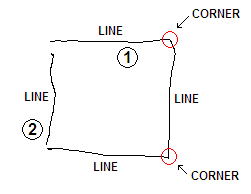
\includegraphics[width=1.8in]{primitive_corners.png}
  \caption{Fragmenting stroke (1) at the two corners indicated breaks the stroke into three primitive lines.}
  \label{fig:primitive_corners}
\end{figure}


\section{Related Work}

Yu and Cai \shortcite{Yu03} designed a corner finder based on curvature and direction changes within a stroke. Their system does not consider speed data because they believe it adds too much noise, whereas our fragmenter filters out noise in order to utilize pen speed.

More related work here...

We designed our fragmenter based on work by Sezgin et al. and Stahovich ~\shortcite{Sezgin01,Stahovich04}. They fragmented strokes by employing pen speed and curvature data, but
they only used average based filtering to smooth their data and reduce noise. Average based filtering smooths a set of data by setting the value at a given index to the average of the values to both sides. Our Approach section discusses their work in detail and evaluates why average based filtering alone is insufficient in curtailing noise.


\section{Fragmenter Approach}

After a sketch is drawn individual pen strokes are analyzed to determine points of minimal pen speed and maximal stroke curvature. These points of 
slow speed and high curvature indicate possible break points of a stroke as users tend to slow their pens when drawing intentional corners.

We construct an initial corner estimation by collecting all the speed local minima points below a certain threshold, and all the curvature local maxima 
points above a certain threshold. We set our speed threshold to be 25\% of the average speed of a stroke and our curvature threshold equal to 0.45 degree/pixel. 
Both of these values were empirically determined and fine-tuned for our hardware.

The stroke in Figure \ref{fig:stroke_example} is part of a digital OR gate and drawn using a Compaq tc4200 Tablet PC.  We extracted speed and curvature data from the stroke and plotted the results in Figure \ref{fig:unfiltered}. %The fragmenter found two potential corners below the speed threshold, and two potential corners above the curvature threshold.

\begin{figure}[t]
  \centering
  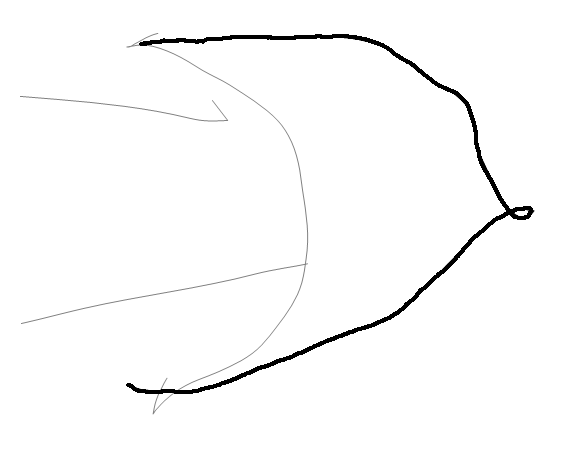
\includegraphics[width=1.4in]{stroke_example_traced.png}
  \caption{An example arched stroke that is part of a digital OR gate.}
  \label{fig:stroke_example}
\end{figure}

\begin{figure}[t]
  \centering
  \subfigure[Pen Speed]
  {
    \label{fig:speed_dirty}
    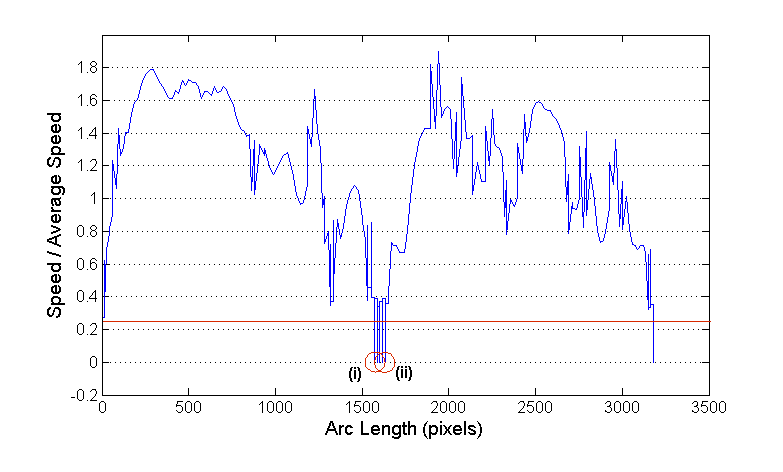
\includegraphics[width=3.4in]{speed_dirty_corners.png}
  }
  \subfigure[Stroke Curvature]
	{
	  \label{fig:curvature_dirty}
	  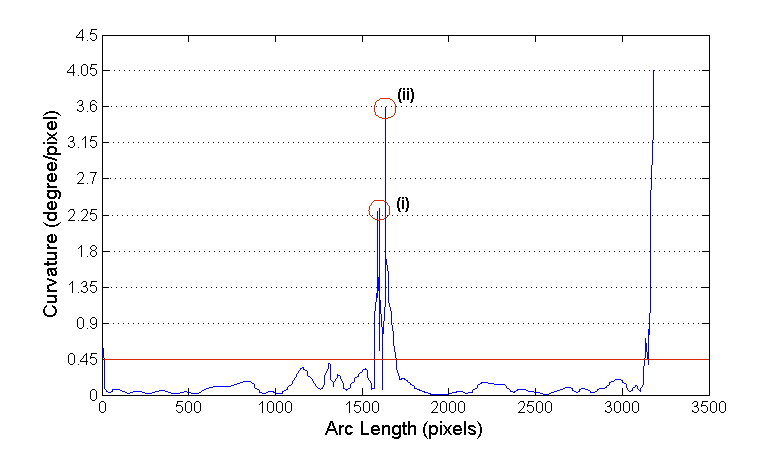
\includegraphics[width=3.4in]{curvature_dirty_corners.png}
  }
  \caption{Speed and curvature graphs for the stroke in Figure \ref{fig:stroke_example}. Thresholds of 25\% of the average speed and 0.45 degree/pixel are indicated by their respective lines, and found corners are indicated by circles.}
  \label{fig:unfiltered}
\end{figure}

%(NOTE: Improve segue into this, reword next paragraph(s) to make less boring)

We then narrow down the initial corner candidates and obtain our final corner set for a stroke through algorithms to merge segments of similar arc, segments of insufficient 
length, and points of close distance. These algorithms are discussed in more detail by Stahovich ~\shortcite{Stahovich04}.

In order to calculate the speed of a stroke we needed to know the arc length, or path distance, of a point on the stroke as well as the time the point was created. The path distance $d_i$ for an individual point $P_i$ is the sum of the Euclidean distances between all previous points:

\begin{equation}
d_i = \sum^{i}_{j=1} \sqrt{(x_j - x_{j-1})^2 + (y_j - y_{j-1})^2}
\end{equation}

\noindent where $x_j$ and $y_j$ correspond to the point $P_j$'s $(x,y)$ coordinates, respectively.

The speed $s_i$ of a point is calculated as the average $distance/time$ speed between the two surrounding points of at the index:

\begin{equation}
s_i = \frac{d_{i+1} - d_{i-1}}{t_{i+1} - t_{i-1}}
\end{equation}

\noindent Using the average speed of the surrounding points helps smooth the pen speed by eliminating slight fluctuations between points.

Curvature is defined as the change in tangent angle, $\theta$, with respect to arc length. Here again we have implemented Sezgin et. al's approach
to curvature. Other computations worked better for calculating curvature of heavily curved objects, such as
circles, but the results tended to fluctuate more when determining the curvature of straight but noisy lines ~\cite{Yu03}.

To find the tangent angle for a specific point we calculate a least squares fit to a window of data points. Our window consists of
eleven data points: our current point, the five points preceding this point, and the five points following this point. A window of
points helps smooth noise in the collected data by reducing individual variations between points. 

Both a least squares line fit and a least squares circle fit are computed for our window, and the better fit is used in the tangent 
calculation. If the least squares line fit is better, then the tangent angle at a given point is equal to the slope of the least squares line fit.
If a least squares circle fit better represents the points, then a tangent line for the current point is taken from the circle and the
tangent angle is the slope of this line.

Once we calculate the tangent angle for each point, we take the curvature at a point $P_i$ to be the slope of the tangent angle versus arc length at index $i$. 
This measures the change in tangent angle as we move from point to point. We again calculate the slope by fitting a least squares line to a window of eleven points
and using the slope of the resulting line.


\section{Analysis}

We analyzed our fragmenter using digital circuit sketches collected from eight undergraduate students. The eight students all had a computer science background, 
but only two students had taken courses heavily emphasizing digital circuitry. None of the students had more than two hours of use on a Tablet PC prior to this test.

Each student was asked to copy two given circuits in Microsoft\textsuperscript{\textregistered} Windows Journal using a Compaq tc4200 Tablet PC. The two circuits to draw
were handed to the users on a sheet of paper and contained simple combinations of wires, OR, AND, NAND, and NOT gates. No drawing constraints were placed upon the user.

The following sectiosn discuss limitations of the current fragmentation system using pen speed and curvature, as well as solutions for these weaknesses.

\subsection{Noise Reduction}

Both Sezgin and Yu's approaches use windows of points when calculating tangent angles and curvatures in order to reduce noise
and improve smoothing. However, relying only on windows of points to improve smoothing is insufficient if a stroke was drawn slowly. Depending on the sampling rate
of hardware, a slowly drawn stroke could record multiple points for a single coordinate.

Overlapping points in a stroke generate numerous problems with our calculations. For example, when we calculate the speed of a point $P_i$, if $P_{i-1}$'s $(x,y)$
coordinates equal $P_{i+1}$'s coordinates, then their path lengths are equal and the speed and $P_i$ is zero. This is a local speed minima, and therefore 
$P_i$ is an initial candidate for a corner point. Multiple subsets of overlapping points within a stroke heavily influence our minima speed calculations and
can produce many false positives.

Overlapping points also affect our least squares fit computations. The least squares algorithms we use try to fit a line or circle to a set of $(x,y)$ points.
The algorithm fits the shape to our 11-point windows, and if many of those coordinates are repetitive we will have a less accurate fit. Tangent angle and
curvature values become more noisy as these slopes fluctuate around clusters of overlapping points.

%(NOTE: Insert least squares graphs here)

Our solution to this problem deals with merging overlapping points into a singular point that preserves all of the relevant information. A sketch drawn in Microsoft\textsuperscript{\textregistered} Windows Journal stores the sketch as a series of strokes that contain points.  Points store their coordinate position and pressure. A larger pressure indicates a more forceful downward pressing of the stylus, and much like an actual marker a more forceful press would
mean a slightly larger width and height for the point. Visually, between two overlapping points, we can only see the point with the largest pressure.

Time information is stored in individual strokes and indicates when the stylus was finally lifted after drawing. We can extrapolate
the information to individual points by using the hardware's sampling rate.

We can now merge overlapping points such that no timing or visual information is lost. A subset of points can only be merged if they have the same $(x,y)$ coordinates
and fall within the same block of time. If those criteria are met we can merge the subset into a singular point, $P_s$, such that:

\begin{enumerate}
  \item The coordinates of the point, $(x_s,y_s)$, equal the coordinates of every point within the subset
  \item The time of $P_s$ equals the time of the final point drawn in the subset, or the point with the largest time.
  \item The pressure of $P_s$ is equal to the maximum point pressure within the subset.
\end{enumerate}

\noindent $P_s$ contains all of the relevant information about the subset. Visual information is preserved since $P_s$ has the same coordinates as well as the largest pressure.  Temporally, we use the final point's time in order to keep the timing information consistent with how we store stroke times; the time marks the instance where the stylus left the point's coordinates. 

Using this individual point instead of a group of overlapping points now eliminates the problems we had with noisy speed and curvature calculations. Speed calculations
will produce fewer zero speeds, and least squares calculations will fit lines and arcs to more diverse point windows. 

Figure \ref{fig:filtered} demonstrates how removing overlapping points from a stroke (Figure \ref{fig:stroke_example}) produces a better overall smoothing of speed and curvature data. Whereas the unfiltered data (Figure \ref{fig:unfiltered}) has a great deal of fluctuation when the stroke is drawn, the filtered data has considerably less noise. We collected data to quantify this smoothing and test how well our filtering reduces false positives.

\begin{figure}[t]
  \centering
  \subfigure[Pen Speed]
  {
    \label{fig:speed_clean}
    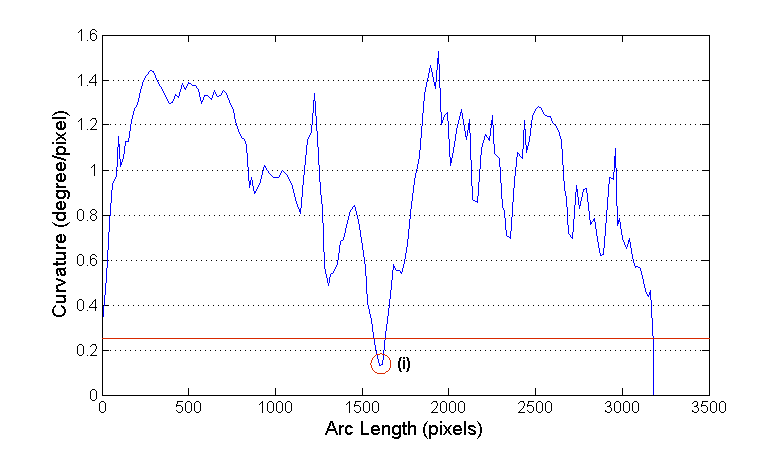
\includegraphics[width=3.4in]{speed_clean_corners.png}
  }
  \subfigure[Stroke Curvature]
  {
    \label{fig:curvature_clean}
    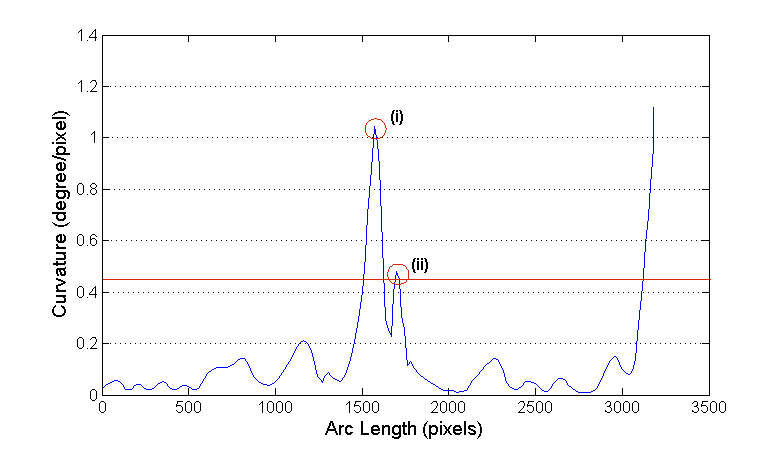
\includegraphics[width=3.4in]{curvature_clean_corners.png}
  }
  \caption{Smoothed speed and curvature graphs for the stroke in Figure \ref{fig:stroke_example}. Overlapping points have been filtered from the stroke
  prior to the speed and curvature calculations.}
  \label{fig:filtered}
\end{figure}

Table \ref{table:filter_table} contains various results from our data collection. The initial number of corners found pertains to the corners found after only checking a stroke's 
speed and curvature against thresholds. If a stroke's speed is below a threshold at a given point, then the point is included in the set of initial corners. Likewise, if
a stroke's curvature is above a threshold at a given point, the point is also included in the set of initial corners. Final corners are the corners remaining after a stroke's initial corners are merged and eliminated using techniques discussed by Stahovich ~\shortcite{Stahovich04}.

Filtering out overlapping points reduces the number of initial corners found by approximately 50\%. Since our fragmenter rarely misses a corner (false negative) around 50\% of the initial corners on the unfiltered data are false positives from noise. Even after merging and eliminating initial corners, the filtered data finds over 50\% less false positives than when we do not remove overlapping points.

Removing extraneous points also reduces the number of total points in the sketches by over 20\% without a loss of data. Algorithms that have an asymptotic time determined by
the number of points in a sketch will greatly benefit from our significant data compression.


\subsection{Constant Factors}

Fragmenting with pen speed and curvature is also limitated by the use of constant thresholds. Fragmentation accuracy is very sensitive to changes in the system defined thresholds for minima speed and maxima curvature. 

We chose our current thresholds of 25\% of the average stroke speed and 0.45 degree/pixel because those thresholds work best for our collected data on the hardware we are using. Yet, if we gathered more data slightly different thresholds might improve our overall accuracy. Different drawing domains require different thresholds as well. A domain consisting of only lines, such as arrows and boxes, would rely heavily on curvature information since corners should only be found where two lines are joined with a significant angle. A domain where strokes are drawn at an relatively even speeds with little curvature variation, such as sinusoids, would require more relaxed thresholds in order to detect any corners (Figure \ref{fig:domain_example}).

\begin{figure}[b]
  \centering
  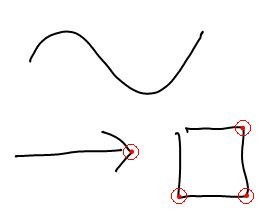
\includegraphics[width=1.4in]{curve_arrow.png}
  \caption{An example of how the current thresholds of 25\% average pen speed and 0.45 degree/pixel curvature do not work for all domains.
  Found corners are marked by circles.}
  \label{fig:domain_example}
\end{figure}

Changing our thresholds slightly produces different fragmentation results. Table \ref{table:threshold_table} tabulates our fragmenter's output when executed on the collected user
data with varying thresholds. Tighter thresholds of 10\% average speed and 0.60 degree/pixel curvate produced a fragmentation with less initial corners found than with our standard thresholds, but the fragmenter also had many more false negatives. Likewise, looser thresholds of 40\% average speed and 0.30 degree/pixel curvature finds more initial corners than our standard case but larger numbers of false positives.

The system's performance is also limited by our constant point windows. We use a window of eleven points, or five points to the left and right of a given point, when we calculate curvature information and least squares fits. The size of the window influences how much variation and noise is present in the curvature calculation of a stroke. For example, we graphed the curvature of the stroke in Figure \ref{fig:stroke_example} using windows of 7, 11, and 15 points (Figures \ref{fig:curv_window3}, \ref{fig:curv_window5}, and \ref{fig:curv_window7}). As the window increases, the amount of noise in the data decreases while the overall curvature extrema are dampened. Larger point windows correspond to less change between consecutive least squares fits since each point has less weight.

\begin{figure}[t]
  \centering
  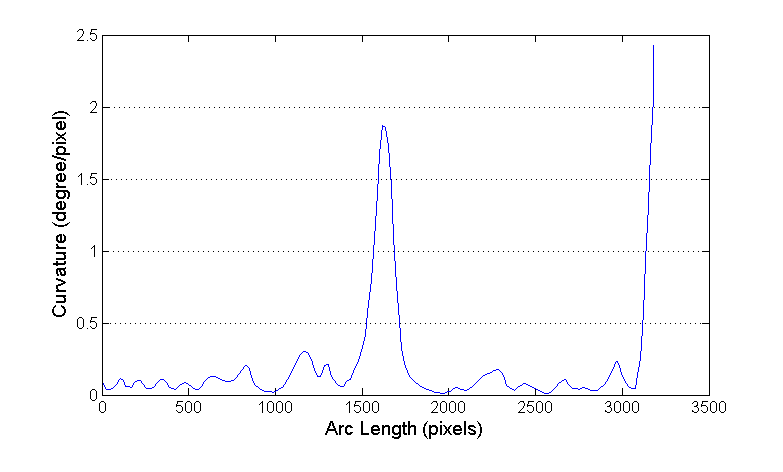
\includegraphics[width=3.4in]{curvature_win3.png}
  \caption{Curvature graph of the stroke in Figure \ref{fig:stroke_example} with a 7-point window. Overlapping points had been filtered out.}
  \label{fig:curv_window3}
\end{figure}

\begin{figure}[t]
  \centering
  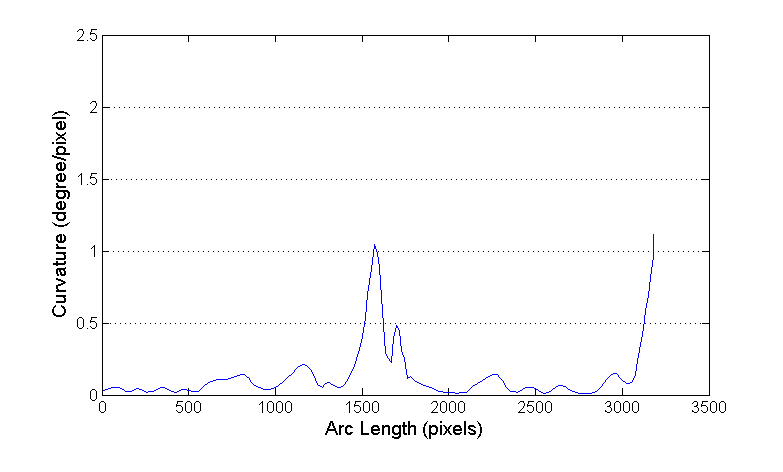
\includegraphics[width=3.4in]{curvature_win5.png}
  \caption{Curvature graph of the stroke in Figure \ref{fig:stroke_example} with an 11-point window. Overlapping points had been filtered out.}
  \label{fig:curv_window5}
\end{figure}

\begin{figure}[t]
  \centering
  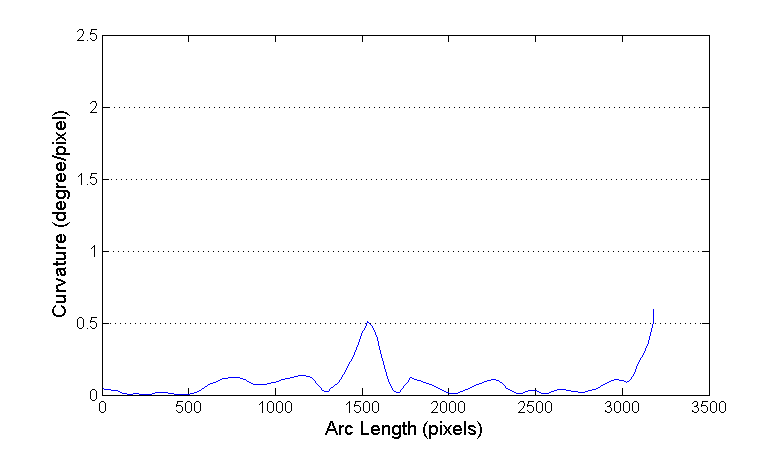
\includegraphics[width=3.4in]{curvature_win7.png}
  \caption{Curvature graph of the stroke in Figure \ref{fig:stroke_example} with a 15-point window. Overlapping points had been filtered out.}
  \label{fig:curv_window7}
\end{figure}

We ran the fragmenter with various window sizes to tabulate how point windows affect the overall fragmentation of a sketch (Table \ref{table:window_table}). The 7-point window
results contain many false positives because the extrema were amplified from our 11-point window standard. Increasing our curvature thresholds to accommodate higher extrema would counteract this to some degree, but 7-point window fits are noisier than 11-point windows in general so more false positives are to be expected. Using a 15-point window produced the best overall fragmentation accuracy with a value of 92.8\%, but it also had 2.6\% false negatives. Our standard fragmentation model had slightly worse overall accuracy with 90.8\%, but we missed a corner only 0.5\% of the time. 

%(NOTE: I know I haven't talked about why we favor false positives yet, but it's discussed in %the Strengths subsection. I'm not sure if I should include that part here instead, or if I %should just not talk about the 15-pt window's accuracy)

\textbf{Solution part:}

Fragmenting by pen speed and curvature is limited by the constant thresholds that are set and requires developers to tweak these values for a particular domain. Can we quantify noise somehow (number of local maxima/minima?) so that we can find thresholds and windows for each sketch individually?

\subsection{Speed Issues}

I haven't even gathered any data for this yet.

\begin{itemize}
  \item Slowly drawn $\rightarrow$ high curvature fluctuation. So many points are close together that a slight speed up or noisy point can alter the curvature.
  \item Fastly drawn $\rightarrow$ any little slowdown is detected if the average speed is very fast. Deliberate, but fast curvature fluctuations are not picked up.
  \item If one part of the stroke is drawn very fast and the other very slow it can greatly affect finding any corners by speed (i.e. lots of symbols drawn in 1 stroke)
\end{itemize}





\subsection{System Strengths}

Even with all of the limitations previously mentioned, using pen speed and curvature to fragment ink strokes produces accurate results. Our fragmenter
obtained an overall 90.8\% accuracy rating when we filtered overlapping points from the strokes, and even without noise reduction the system's accuracy was 84.6\% (Table \ref{table:filter_table}).

This fragmenting technique can also be used in most 2D sketches domains. We applied the fragmentation to digital circuits to see how well the fragmenter could break up
wires and gates. Stahovich had a 95.8\% average fragmentation accuracy when he tested the method on individual symbols and shapes \shortcite{Stahovich04}. 

We previously discussed how using constant thresholds limits the system, but at the same time using system defined thresholds can benefit the developer. A developer could tweak the system to favor false positives or false negatives by lowering or raising threshold values. Our fragmenter implementation favors false positives because we feel it is better to overfragment initially and deal with extraneous data at a later time. If we lower our speed threshold and increased our curvature threshold, we miss more corners and our false negatives increase (Table \ref{table:threshold_table}). Depending on a system's requirements, fragmenting with pen speed and curvature can easily underfragment or overfragment a sketch.

%\section{Future Work}


\section{Conclusion}



%\section{Acknowledgments}

%We'd like to thank all of the computer science students who helped us collect sketch data %during the summer, as well as the E85 students in Spring 2006. We would also like to thank MIT %for their...


\bibliography{fragmenter}
\bibliographystyle{acmsiggraph}
%\bibliographystyle{abbrv}
%\nocite{*}

\clearpage

\begin{table*}[p]
   \centering
   \begin{tabular}{||r||r|r|r||}
	    \hline
	    & Unfiltered Sketches & Filtered Sketches & Difference, \% \\
	    \hline 
	    Total Number of Sketch Points & 75668 & 59128 & 21.9 \\
	    \hline
	    Initial Number of Corners Found & 2537 & 1312 & 48.3 \\
	    \hline
	    Final Number of Corners Found & 225 & 208 & 7.6 \\
	    \hline 
	    False Negatives & 3 & 1 & 66.7 \\
	    \hline
	    False Positives & 37 & 18 & 51.4 \\
	    \hline
	    \hline
	    Actual Number of Corners & 191 & 191 & \\
	    \hline
	    \% False Negatives & 1.6 & 0.5 & \\
	    \hline
	    \% False Positives & 16.4 & 8.7 & \\
	    \hline
	  \end{tabular}
	  \caption{User data fragmented with unfiltered sketches and sketches with removed overlapping points. Thresholds of 25\% average speed and 0.45 degree/pixel
	  curvature were used when gathering this data, as well as an 11-point window.}
	  \label{table:filter_table}
\end{table*}

\begin{table*}[p]
   \centering
   \begin{tabular}{||r||r|r|r||}
	    \hline
	    & 10\% Avg. Speed, & 25\% Avg. Speed & 40\% Avg. Speed \\
	    & 0.60 degree/pixel & 0.45 degree/pixel & 0.30 degree/pixel \\
	    \hline
	    Initial Number of Corners Found & 894 & 1312 & 1628 \\
	    \hline
	    Final Number of Corners Found & 197 & 208 & 252 \\
	    \hline 
	    False Negatives & 12 & 1 & 0 \\
	    \hline
	    False Positives & 18 & 18 & 61 \\
	    \hline
	    \hline
	    Actual Number of Corners & 191 & 191 & 191 \\
	    \hline
	    \% False Negatives & 6.3 & 0.5 & 0.0 \\
	    \hline
	    \% False Positives & 9.1 & 8.7 & 24.2 \\
	    \hline
	  \end{tabular}
	  \caption{User data fragmented with different speed and curvature thresholds. An 11-point window was used for all of these fragmentations.
	  Overlapping points were filtered from the strokes.}
	  \label{table:threshold_table}
\end{table*}

\begin{table*}[p]
   \centering
   \begin{tabular}{||r||r|r|r||}
	    \hline
	    & 7-Point Window & 11-Point Window & 15-Point Window \\
	    \hline 
	    Initial Number of Corners Found & 1605 & 1312 & 1151 \\
	    \hline
	    Final Number of Corners Found & 242 & 208 & 195 \\
	    \hline 
	    False Negatives & 2 & 1 & 5 \\
	    \hline
	    False Positives & 53 & 18 & 9 \\
	    \hline
	    \hline
	    Actual Number of Corners & 191 & 191 & 191 \\
	    \hline
	    \% False Negatives & 1.1 & 0.5 & 2.6 \\
	    \hline
	    \% False Positives & 21.9 & 8.7 & 4.6 \\
	    \hline
	  \end{tabular}
	  \caption{User data fragmented with different point windows. Thresholds of 25\% average speed and 0.45 degree/pixel
	  curvature were used when gathering this data. Overlapping points were filtered from the strokes.}
	  \label{table:window_table}
\end{table*}

\end{document}

% HERE IS HOW TO INSERT A FIGURE
%\begin{figure}[h]
%\centering
%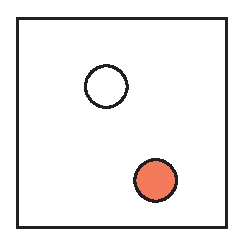
\includegraphics[width=1.5in]{sample.eps}
%\caption{Sample illustration.}
%\end{figure}